\item Quando apenas duas engrenagens estão engrenadas, a engrenagem motriz $A$ e a engrenagem movida $B$ sempre girarão em direções opostas. A fim de fazer com que elas girem na mesma direção, uma engrenagem intermediária $C$ é usada. No caso mostrado, determine a velocidade angular da engrenagem $B$ quando $t=\SI{5}{\second}$, se a engrenagem $A$ parte do repouso e tem uma aceleração angular $\alpha_{A} =(3\,t+2)$ $\SI{}{\radian/\second^{2}}$, onde t é dado em segundos.

\import{../answers/}{answer-2}

\begin{flushleft}
	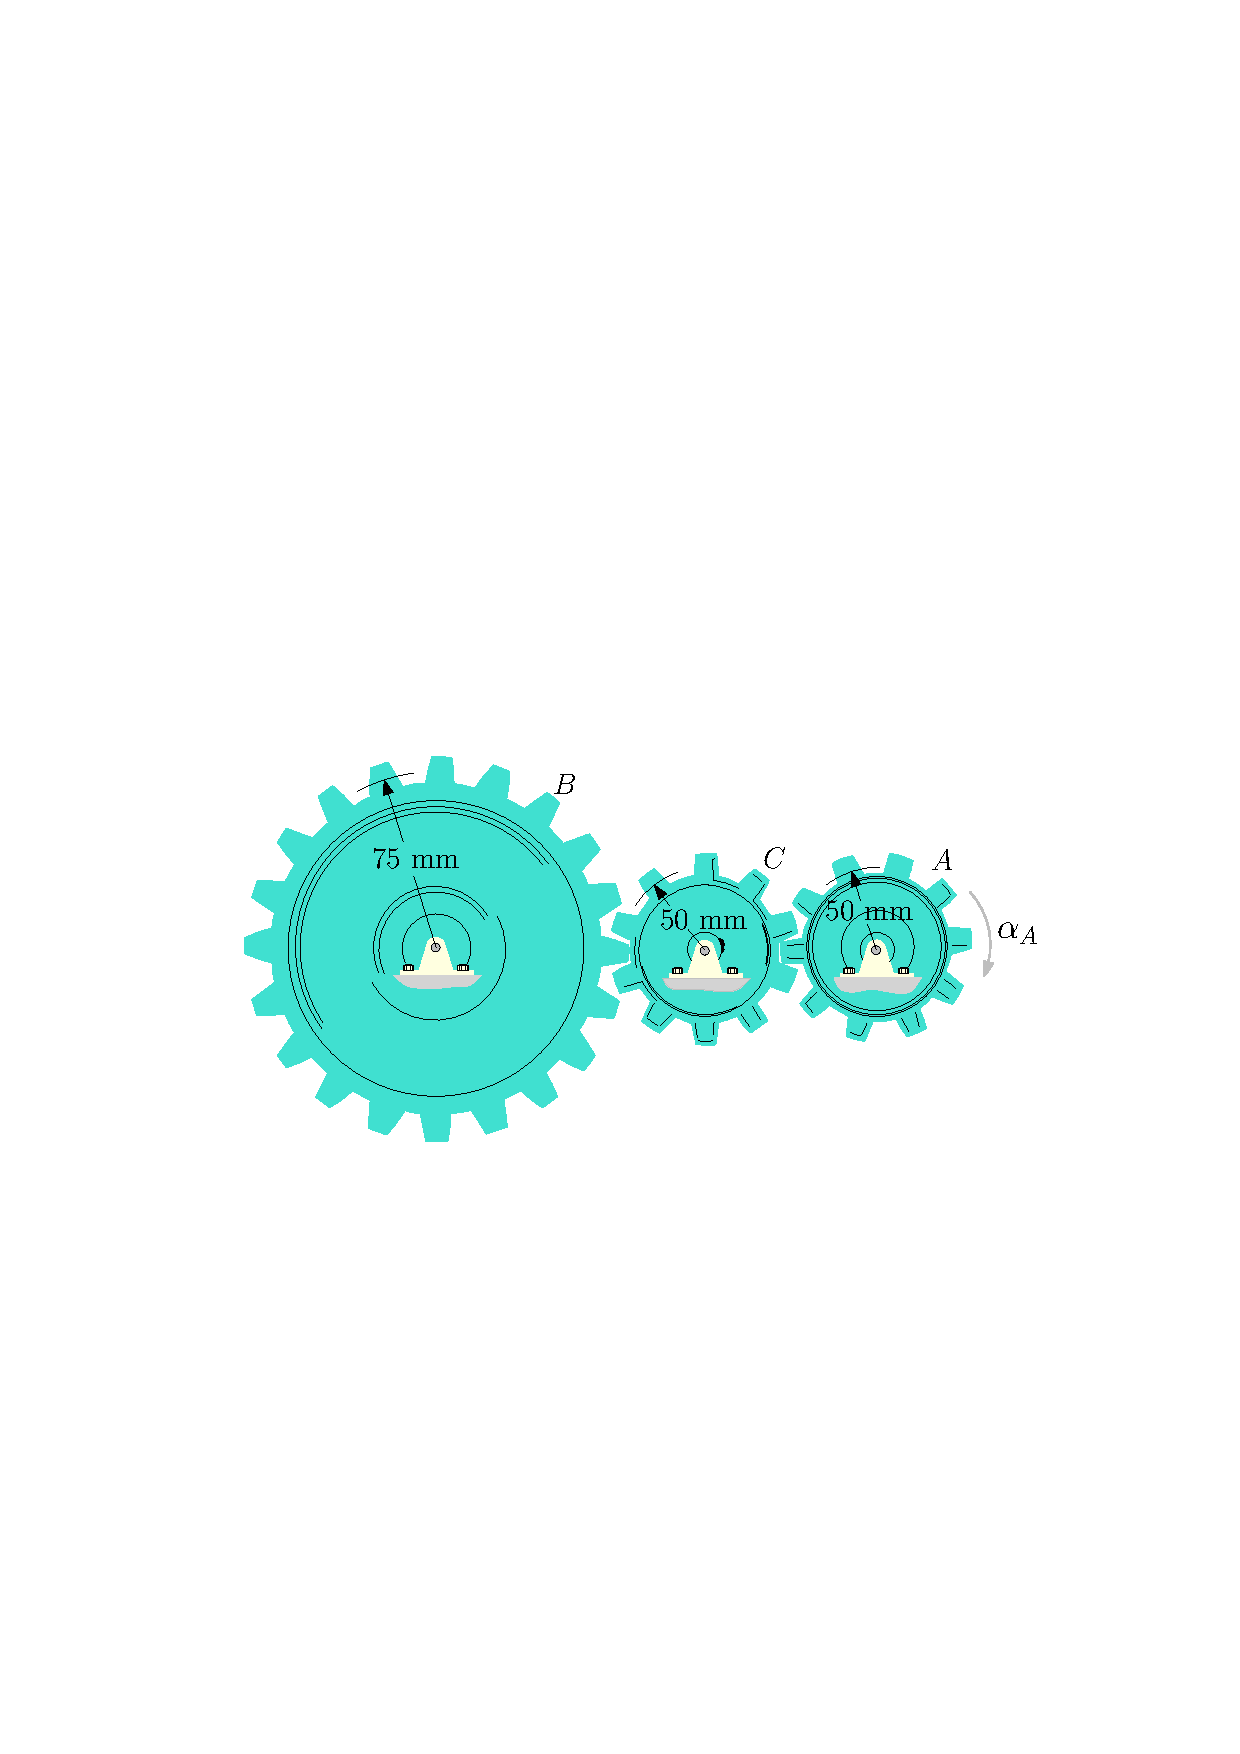
\includegraphics[scale=.85]{images/draw_2}
\end{flushleft}